% exercise sheet with header on every page for math or close subjects
\documentclass[12pt]{article}
\usepackage[utf8]{inputenc} 
\usepackage{latexsym} 
\usepackage{multicol}
\usepackage{fancyhdr}
\usepackage{amsfonts} 
\usepackage{amsmath}
\usepackage{amssymb}
\usepackage{enumerate}
\usepackage{listings}
\usepackage{graphicx}

% Shortcuts for bb, frak and cal letters
\newcommand{\E}{\mathbb{E}}
\newcommand{\V}{\mathbb{V}}
\renewcommand{\P}{\mathbb{P}}
\newcommand{\N}{\mathbb{N}}
\newcommand{\R}{\mathbb{R}}
\newcommand{\C}{\mathbb{C}}
\newcommand{\Z}{\mathbb{Z}}
\newcommand{\Pfrak}{\mathfrak{P}}
\newcommand{\Pfrac}{\mathfrak{P}}
\newcommand{\Bfrac}{\mathfrak{P}}
\newcommand{\Bfrak}{\mathfrak{B}}
\newcommand{\Fcal}{\mathcal{F}}
\newcommand{\Ycal}{\mathcal{Y}}
\newcommand{\Bcal}{\mathcal{B}}
\newcommand{\Acal}{\mathcal{A}}


% Formatierung
\topmargin -2cm 
\textheight 24cm
\textwidth 16.0 cm 
\oddsidemargin -0.1cm

\setlength{\parindent}{0pt}  % !!!!!!! Hier werden leerzeilen erlaubt ohne dass Latex automatisch einrueckt! !!!!!!! %


\graphicspath{ {images/} }


\begin{document}

% Titel
%\title{\textsc{Hacking}\\ \textsc{Abgabe 0}\\{ \normalsize Gruppe X \hfill Daniel Schäfer (2549458)\\ \hfill Anderer}}
%\maketitle  

% alternativer Titel
\noindent
{\Large \textbf{High-level Computer Vision}} \hfill \textbf{26.05.2016}\\
{\Large \textbf{Exercise 3}} 
\raggedleft \hfill Guillermo Reyes (2556018)\\
\hfill Daniel Schaefer (2549458)\\
\hfill Marc Tonsen (2537359)\\
\hfill Dominik Weber (2548553)\\

\pagenumbering{gobble}
\raggedright


\section*{Code Annotations}




\section*{Question 1: Support Vector Machines}

\begin{enumerate}[a)]
	\setcounter{enumi}{1}
	\item 	
        \textbf{Modify the last two parameters of} \verb!get\_train\_dataset\_2d.m! \textbf{in order to make the classification problem linearly non-separable. Run your visualization for different values of parameter C and comment on its role in the SVM classification algorithm.}\\
        
        	\begin{figure}[h]			
        		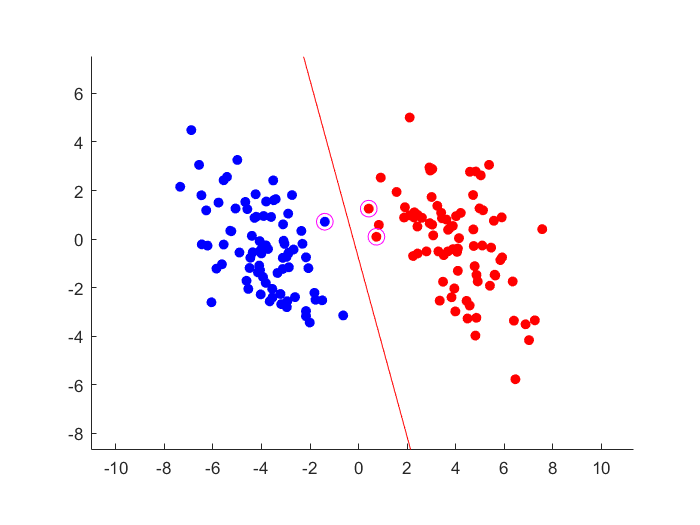
\includegraphics[width=0.5\textwidth]{1b_separable}
        		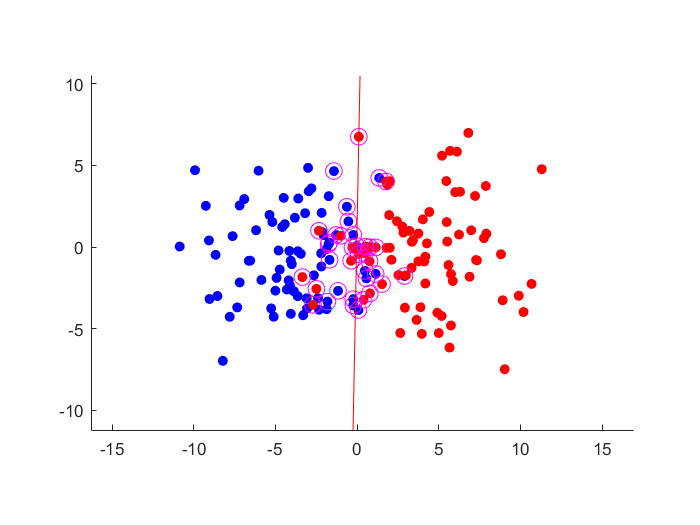
\includegraphics[width=0.5\textwidth]{1b_non-separable}
        		\caption{\textit{Left}: SVM for linearly separable data with default parameters. $ \sigma_1=1.5, \sigma_2=5 $. \textit{Right}: SVM for linearly non-separable data. The same parameters are used to generate the data except that $ \sigma_1=10 $ and $\sigma_2=10 $ and $C=100$ }
        	\end{figure}
        In Figure 1 we can see on the left, the linearly separable data of two distributions. The best fit for a separating hyperplane results in a margin of 1.88 and 3 support vectors. By making the the sigmas of the distributions large enough, we are effectively making the data more spread, and thus, the two distributions overlap. the result is the image on Figure 1, right.  By generating the data with $\sigma_1=10 $ and $\sigma_2=10 $ the the two distributions share a common region in space and are therefore no longer separable. How ever by using a soft margin SVM we can still fit the hyperplane that best "splits" the data i.e. the one with largest margin. In this case we can get a margin of about 3.45 with 38 support vectors.
        
        
           	\begin{figure}[h]			
          		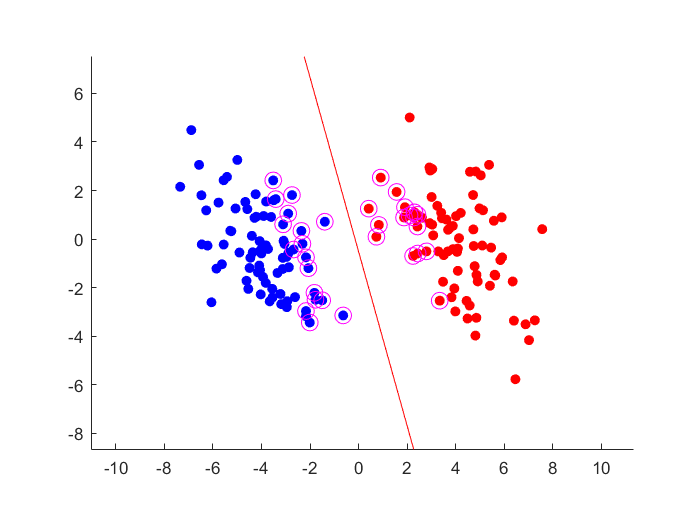
\includegraphics[width=0.5\textwidth]{1b_separableC005}
           		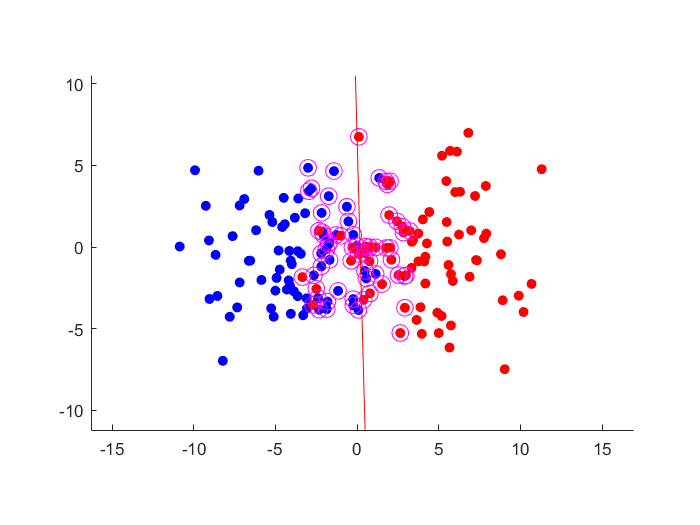
\includegraphics[width=0.5\textwidth]{1b_non-separableC005}
          		\caption{\textit{Left}: SVM for linearly separable data with default parameters. $ \sigma_1=1.5, \sigma_2=5, C = .005$ The margin is 5.48 and there are 34 support vectors. \textit{Right}: SVM for linearly non-separable data. The same parameters are used to generate the data except that $ \sigma_1=10, \sigma_2=10, C=.005 $. Here the margin is around 6.1 and there are 66 support vectors }
           	\end{figure}
        
		The parameter C is used in the minimized loss function to tune the importance of the sum of $\xi$'s. A high value for C would put a lot of importance on them and would therefore force them to take very small values. Therefore, the higher the value of C is, the closer the performance comes to that of a hard-margin SVM. If C has a small value this would soften the margin and would also allow support vectors inside the margin, even when the data is linearly separable. In Figure 2, left we can see and example if this: the data was generated by the same parameters as in Figure 1, but the selected C is .005, which allows the margin to grow to 5.48 and the use of 34 support vectors (against 3 used before). In Figure 2, right we also see how setting the parameter C to a lower value allows the margin to be softer. In conclusion C influences how soft the margin of the SVM is for both: linearly separable and non-linearly separable data.
\end{enumerate}

\newpage
\section*{Question 3: Performance Evaluation}
\begin{enumerate}[a)]
	\setcounter{enumi}{3}
	

	\item
        \textbf{Write a summary of your observations and submit it along with the corresponding RPC curves}\\
        %TODO

	\item 
        \textbf{How could you use the system to solve the detection problem in which you are given an image of arbitrary size and the task is to find the position of the people in it?}\\
        %TODO

\end{enumerate}


\end{document}
